\documentclass[11pt]{article}
\usepackage{amsmath}
\usepackage{graphicx}
\usepackage{float}
\usepackage{blindtext}
\usepackage{subcaption}
\usepackage[a4paper,width=180mm,top=22mm,bottom=22mm]{geometry}
\usepackage{fancyhdr}
\usepackage{longtable}
\usepackage[
    backend=biber,
    style=ieee
]{biblatex}
\usepackage{xcolor}
\usepackage{soul}
\usepackage{listings}

\newcommand{\hlc}[2][yellow]{{%
    \colorlet{foo}{#1}%
    \sethlcolor{foo}\hl{#2}}%
}


\addbibresource{report.bib}

\graphicspath{ {./images/} }

\pagestyle{fancy}
\fancyhead[C]{EEE3027}
\fancyhead[L]{EEE3027 Final Essay}
\fancyhead[R]{16th of May}

\cfoot{} % get rid of the page number 
\fancyfoot[L]{6596386}
\fancyhead[C]{}
\fancyfoot[R]{\thepage}

\begin{document}
\begin{titlepage}
    \begin{center}
    
\includegraphics[width=\textwidth]{Logo.png} % also works with logo.pdf
    \vfill
    \Huge
    \textbf{EEE3027: Final Essay}
    \vfill
    \huge
    \vspace{1cm}
    \Large
    16th of May 2023\\
    URN: 6596386\\
    \vfill
    \vfill
    \Large
    School of Computer Science and Electronic Engineering\\
    Faculty of Engineering and Physical Sciences\\
    University of Surrey\\
    \end{center}
\end{titlepage}

\renewcommand{\thesection}{\Alph{section}}
\renewcommand{\thesubsection}{\Alph{section})\alph{subsection}}

\pagenumbering{Roman}
%\begin{abstract}

\vspace{1cm}
%\end{abstract}
\tableofcontents
\pagebreak

\pagenumbering{arabic}
\section{System on a Chip Interfacing}
\subsection{JTAG Advantages}
As chips have become denser, directly probing pins, such as with the old bed-of-nails technique, is no longer possible, yet accessing these pins is vital for testing.
This is the problem the Joint Test Action Group set out to solve with JTAG, which is a specification for accessing on-ship resources and boundary-scan hardware testing on the board\cite{jtag_tutorial}.
Without boundary-scanning, the only test option is functional, which requires massive amounts of test cases to exhaust all possibilities and does not help find the cause of a failure.
Meanwhile, JTAG's boundary scan enables one to control and monitor individual IO pins, allowing for structural tests. 
Structural tests will help find assembly defects, such as shorts, and run much quicker as they are non-exhaustive.

JTAG also offers other benefits, such as monitoring systems during operation without disrupting them and even testing systems that are otherwise non-functional\cite{Corelis}.
This is because JTAG is independent of the system and accessible via just four pins (depending on specification).
As the logic and pins are part of the IC, JTAG will allow for testing throughout a product's life cycle.
Engineers can use the interface during prototyping, production, and after deployment\cite{Corelis}.
JTAG also daisy chains, allowing multiple devices within a system to be tested with one interface.

(208)


\subsection{JTAG Functionality}
The JTAG implementation shown in Figure 1 of the essay brief connects to the internal bus of the ARM Cortex-M0 SoC.
This connection enables the JTAG interface to control and monitor the data on that bus, allowing one to shift in a test pattern to test
the NVIC, processor core, debug subsystem, memory and peripherals, or any combination thereof. 

This sort of boundary testing is done via a path of interconnected shift-register cells on each signal pin in the bus, which are controlled via the Test Access Port (TAP) of the JTAG.
The TAP has four core control signals\cite{JTAG}:
\begin{itemize}
    \item TCK, clock to synchronize operation
    \item TMS, mode select line
    \item TDI, input shifted into cells on the rising edge
    \item TDO, output shifted out of cells on the falling edge 
    \item (Optional) TRST, a reset for the state machine 
\end{itemize}

Creating this functionality in VHDL is done by creating a state machine, shown in Figure \ref{fig:sm}, which is controlled by the value of TMS during the rising edge of TCK.
The state machine has two paths to capture and control the data on the instruction registers (IR) or the data registers (DR).

\begin{figure}[H]        
    \centering
    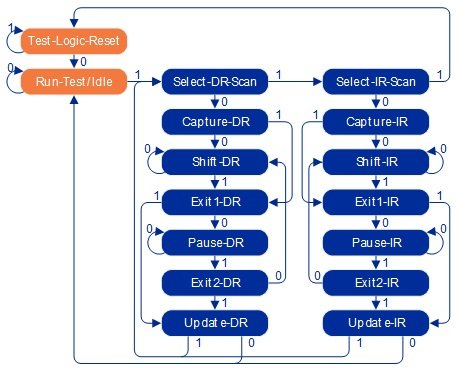
\includegraphics[width=\textwidth]{JTAG-state-machine-diagram1.jpg}
    \caption{JTAG State Machine Diagram from Corelis\cite[Corelis]}
    \label{fig:sm}
\end{figure} 

The cells must also be created in VHDL using multiplexers and latches. 
These cells have a parallel input and output, which allow for the regular operation of the device, and shift inputs and outputs, which are used during tests to load data in or read data out.

(235)


\subsection{VHDL Implementation}

\subsection{Calculations Single Stage}
\subsection{Calculations Four Core}

\section{Design Challenge}
\subsection{Architecture and Block's Design}
\subsection{VHDL Implementation}

\pagebreak
\appendix
\renewcommand{\thesection}{\Roman{section}}
\section{References}
\printbibliography[heading=none]

\end{document}